%%% SVN stuff
\svnidlong
{$HeadURL: https://svn.riouxsvn.com/kneadlatxinputs/ExampleArtifactFolders/5-SSDD/SSDD_Chapter_04.tex $}
{$LastChangedDate: 2024-02-23 23:39:02 -0500 (Fri, 23 Feb 2024) $}
{$LastChangedRevision: 81 $}
{$LastChangedBy: KneadProject $}
\svnid{$Id: SSDD_Chapter_04.tex 81 2024-02-24 04:39:02Z KneadProject $}


\chapter{System Architectural Design}
\label{loc:SystemArchitecturalDesign}
% \DIDINFO{SSDD-4.0.0 :: This section shall be divided into the following paragraphs to describe the system architectural design. 
If part or all of the design depends upon system states or modes, this dependency shall be indicated. If design information falls into more than one paragraph, it may be presented once and referenced from the other paragraphs. 
Design conventions needed to understand the design shall be presented or referenced.
Note: For brevity, this section is written in terms of organizing a system directly into Hardware Configuration Items (HWCIs), Computer Software Configuration Items (CSCIs), and manual operations, but should be interpreted to cover organizing a system into subsystems, organizing a subsystem into HWCIs, CSCIs, and manual operations, or other variations as appropriate.}

This chapter describes the system architectural design for the \ThisSystem. An overview of all system components is shown in Figure~\ref{fig:SYS-O}

\begin{figure}[htbp]
	\centering
		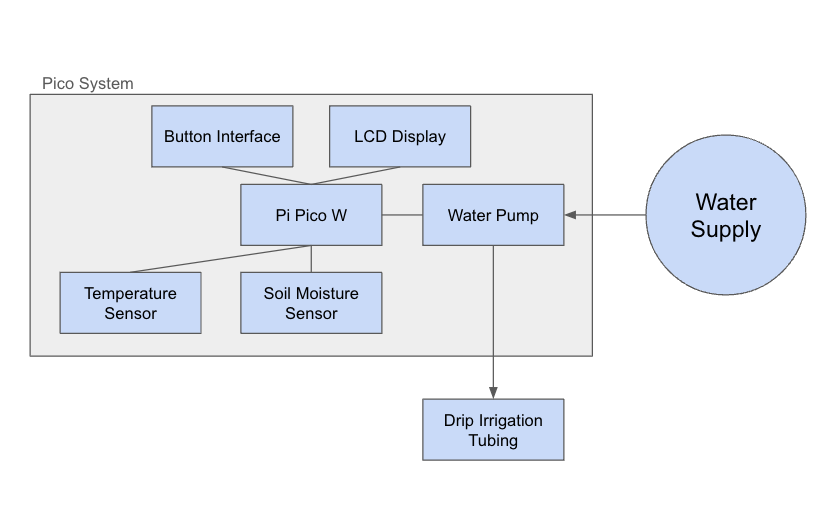
\includegraphics[width=6.5in]{./images/system_overview.png}
	\caption[System Architectural Overview]{System Architectural Overview Diagram}
	\label{fig:SYS-O}
\end{figure}

\section{System Components}
\label{loc:SystemComponents}
% \DIDINFO{SSDD-4.1.0 :: This section shall
\begin{itemize}
\item Identify the components of the system (HWCIs, CSCIs, and manual operations). Each component shall be assigned a project-unique identifier. Note: a database may be treated as a CSCI or as part of a CSCI.
\item Show the static (such as “consists of’) relationship(s) of the components. Multiple relationships may be presented, depending on the selected design methodology.
\item State the purpose of each component and identify the system requirements and system-wide design decisions allocated to it. (Alternatively, the allocation of requirements may be provided in 5.a).
\item Identify each component’s development status/type, if known (such as new development, existing component to be reused as is, existing design to be reused as is, existing design or component to be reengineered, component to be developed for reuse, component planned for Build N, etc.) For existing design or components, the description shall provide identifying information, such as name, version, documentation references, location, etc.
\item For each computer system or other aggregate of computer hardware resources identified for use in the system, describe its computer hardware resources (such as processors, memory, input/output devices, auxiliary storage, and communications/network equipment). Each description shall, as applicable, identify the configuration items that will use the resource, describe the allocation of resource utilization to each CSCI that will use the resource (for example, 20% of the resource’s capacity allocated to CSCI 1, 30% to CSCI 2), describe the conditions under which utilization will be measured, and describe the characteristics of the
resources.
\item Present a specification tree for the system, that is, a diagram that identifies and shows the relationships among the planned specifications for the system components.
\end{itemize}
}

This section lists and describes the system components.

\subsection{Raspberry Pi Pico W}

\begin{description}
    \item[Project Unique ID] \textbf{Pico\textunderscore 1}
    \item[Relationships] 
    \item[Purpose] The Raspberry Pi Pico W is the microcontroller of the entire \ThisSystem. Satisfies requirement 3.10.1.1.
    \item[Development Status] Existing
    \item[Description] Raspberry Pi Pico W
\end{description}

\subsection{Temperature Sensor}

\begin{description}
    \item[Project Unique ID] \textbf{Sense\textunderscore 1}
    \item[Relationships] Interacts with Pico\textunderscore 1
    \item[Purpose] The temperature sensor measures environmental temperature data. Satisfies requirement 3.2.1.4.
    \item[Development Status] Existing
    \item[Description] BME280 Temperature Sensor
\end{description}

\subsection{Soil Moisture Sensor}

\begin{description}
    \item[Project Unique ID] \textbf{Sense\textunderscore 2}
    \item[Relationships] Interacts with \textbf{Pico\textunderscore 1}
    \item[Purpose] The soil moisture sensor measures the soil moisture of the user's garden. Satisfies requirement 3.2.1.5.
    \item[Development Status] Existing
    \item[Description] I2C Capacitive Moisture Sensor
\end{description}

\subsection{Water Pump}

\begin{description}
    \item[Project Unique ID] \textbf{Pump\textunderscore 1}
    \item[Relationships] Controlled by \textbf{Pico\textunderscore 1}
    \item[Purpose] The water pump pumps water from the water supply to the drip irrigation tubing. This is how the irrigation system activates. Satisfies requirement 3.2.1.2.
    \item[Development Status] Existing
    \item[Description] US Solar Pump B3A 5V PWM Circulating Pump
\end{description}

\subsection{Button Interface}

\begin{description}
    \item[Project Unique ID] \textbf{Int\textunderscore 1}
    \item[Relationships] Interacts with \textbf{Pico\textunderscore 1} and \textbf{Int\textunderscore 2}
    \item[Purpose] The button interface controls mode changes for \ThisSys. Satisfies requirement 3.2.1.6.
    \item[Development Status] Existing
    \item[Description] GPIO Pin Buttons
\end{description}

\subsection{LCD Display}

\begin{description}
    \item[Project Unique ID] \textbf{Int\textunderscore 2}
    \item[Relationships] Interacts with \textbf{Pico\textunderscore 1} and\textbf{Int\textunderscore 1}
    \item[Purpose] The LCD Display displays the active mode for \thisSys. Satisfies requirement 3.2.1.7.
    \item[Development Status] Existing
    \item[Description] Adafruit Standard HD44780 LCD
\end{description}

\subsection{Drip Irrigation Tubing}

\begin{description}
    \item[Project Unique ID] \textbf{Out\textunderscore 1}
    \item[Relationships] Connected to \textbf{Pump\textunderscore 1}
    \item[Purpose] The drip irrigation tubing control how much water leaves the irrigation system. Satisfies requirement 3.2.1.1.
    \item[Development Status] Existing
    \item[Description] Rain Bird Drip Irrigation Tubing
\end{description}


\section{Concept of Execution}
\label{loc:ConceptOfEExecution}
\DIDINFO{SSDD-4.2.0 :: This section shall describe the concept of execution among the system components. 
It shall include diagrams and descriptions showing the dynamic relationship of the components, that is, how they will interact during system assembly, storage, deployment, and operation, including, as applicable, flow of execution control, data flow, dynamically controlled sequencing, state transition diagrams, timing diagrams, priorities among components, handling of interrupts, timing/sequencing relationships, exception handling, concurrent execution, dynamic allocation/deallocation, dynamic creation/deletion of objects,
processes, tasks, assembly, storage, deployment, and other aspects of dynamic behavior.}

This section describes the concept of execution based on the system components.


\section{Interface Design}
\label{loc:InterfaceDesign}
\DIDINFO{SSDD-4.3.0 :: This section shall be divided into the following subparagraphs to describe the interface characteristics of the system components. It shall include both interfaces among the components and their interfaces with external entities such as other systems, configuration items, and users. Note: There is no requirement for these interfaces to be completely designed at this level; this paragraph is provided to allow the recording of interface design decisions made as part of system architectural design. If part or all of this information is contained in Interface Design Descriptions (IDDs) or elsewhere, these sources may be
referenced.
\begin{description}
\item[Interface identification and diagrams] This paragraph shall state the project-unique identifier assigned to each interface and shall identify the interfacing entities (systems, configuration items, users, etc.) by name, number, version, and documentation references, as applicable. The identification shall state which entities have fixed interface characteristics (and therefore impose interface requirements on interfacing entities) and which are being developed or modified (thus having interface requirements imposed on them). One or more interface diagrams shall be provided, as appropriate, to depict the interfaces.
\item[Unique Interface Descriptions] These subsections shall identify an interface by project-unique identifier, shall briefly identify the interfacing entities, and shall be divided into paragraphs as needed to describe the interface characteristics of one or both of the interfacing entities. If a given interfacing entity is not covered by this \SSDD (for example, an external system) but its interface characteristics need to be mentioned to describe interfacing entities that are, these characteristics shall be stated as assumptions or as “When [the entity not covered] does this, [the entity that is covered] will.. ..” This paragraph may reference other documents (such as data dictionaries, standards for protocols, and standards for user interfaces) in place of stating the information here. The design description shall include the following, as applicable, presented in any order suited to the information to be provided, and
shall note any differences in these characteristics from the point of view of the interfacing entities (such as different expectations about the size, frequency, or other characteristics of data elements).
\end{description}
}

This section describes the internal and external interface design based on the system components.


\subsection{Interface One}
\label{loc:InterfaceOne}
\input{DIDINFO_Snippets/SSDD/SSDD_4.3.1_DIDINFO.tex}

This section describes the internal and external interface design based on the system components.

\subsection{Interface Two}
\label{loc:InterfaceTwo}
%\input{DIDINFO_Snippets/SSDD/SSDD_4.3.1_DIDINFO.tex}

This section describes the internal and external interface design based on the system components.
